\chapter{光的初步知识}

一道闪电划破了黑暗的天空,接着听到了远处传来的隆隆的雷声。
为什么我们总是先看见闪电,而后才听到雷声呢?

从镜子里可以看到自己的像。镜子里的像,既不放大,也不缩小,跟自己一模一样。这是为什么呢?

你注意观察过浸入水中的物体吗?例如插入水中的一支筷子,从水面上看去,在水中的那部分向上折了。这又是什么道理呢?

上面这几个问题都是跟光有关的现象。跟光有关的现象,在自然界和日常生活中随处可见,
在生产技术和科学研究中也经常利用。这一章,我们就来学习有关光的一些知识。

\section{光的直线传播}\label{sec:1-1}

光是从一些物体发出来的。例如太阳、电灯、蜡烛的火焰等都能够发光。
这些能发光的物体叫做\textbf{光源}。光源发出来的光是怎样向周围传播的呢?

打扫房间的时候,如果有太阳光穿过窗户射进屋子里,照着飘浮的灰尘,会看到光通过的路线是直的。
穿过云隙的太阳光,黑夜里手电筒的光,通过的路线也是直的。这些现象表明,光在空气里是沿直线传播的。

光不仅能在空气里传播,而且还可以在水、玻璃等透明物质里传播。
实验表明,光在任何一种透明物质里传播的路线都是直的。
但是,如果光从一种物质(例如空气)进入另一种物质(例如水或玻璃),它的传播方向通常会改变。
因此,应该说:

\textbf{光在同一种物质里传播的路线是直的}。

通常所说的光线,指的是光通过的路线。所以,上面的结论可以这样说:
\CJKunderwave{在同一种物质里,光线是直的}。

光从光源发出来,照射到物体,需要时间吗?
很早以前,人们认为光的传播是不需要时间的。
根据日常经验,这种看法似乎是对的。
当你打开电灯的时候,整个房间几乎同时都被照亮了。
你觉察不出离电灯近的地方比远的地方会早亮一些。

\begin{enhancedline}[1ex]
但是,实际上光是以一定的速度传播的。
只是由于光的速度非常大,通过不太长的距离需要的时间非常短,因此不易觉察到。
直到十七世纪后半期,人们才第一次测出了光的速度。
现在我们知道,光在真空中的速度是 $3 \times 10^5 \qmmm$。
这个速度相当于一秒钟绕地球赤道七圈半。
光在真空中的速度最大,在空气中的速度跟在真空中的差不多。
因此通常认为光在空气中的速度也是 $3 \times 10^5 \qmmm$。
光在水里的速度大约是空气里的 $\dfrac{3}{4}$。
在玻璃里的速度比在水里的还小。
\end{enhancedline}

光比声音的传播快得多。声音在空气里的速度是 $340\mmm$。
现在你就会明白,虽然闪电和雷声是同时发生的,但是我们却先看见闪电后听到雷声。

\section*{阅读材料}

在我国古书《墨经》中,记载了当时墨家学派的代表人物墨瞿〈约公元前468 ~ 公元前376 )
和他的学生做的世界上最早的小孔成像实验。

\begin{figure}[htbp]
    \centering
    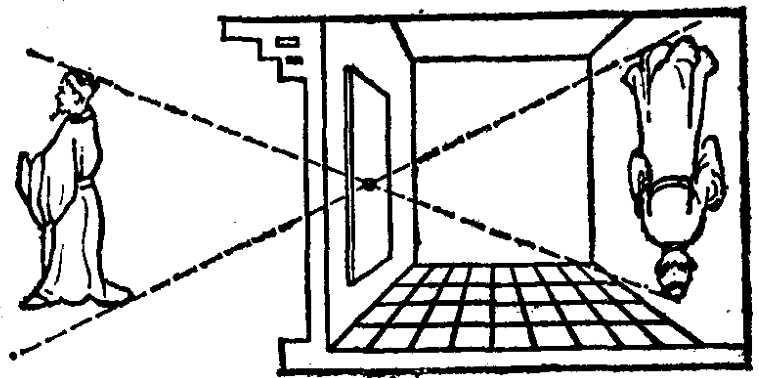
\includegraphics[width=0.7\textwidth]{../pic/czwl2-ch1-1}
    \caption{小孔成像}\label{fig:1-1}
\end{figure}

在一间黑暗的小屋朝阳的墙上开一个小孔。在屋外,小孔的前方站着一个人。
这时屋里相对的墙上就出现了一个倒立的人像〈图 \ref{fig:1-1})。
为什么会出现这奇怪的现象呢?书中解释说,这是因为光象射箭一样,是直线行进的。
从人体上部射来的光,通过小孔,投射在下边;
从人体下部射来的光,通过小孔,投射在上边,这就形成了倒立的像。
并且还指出,人的位置离墙壁由远而近,它的像也由小变大,倒立在墙上。

这个实验到现在已有二千四五百年。
《墨经》在解释小孔成像时明确提出了光的传播路线是直的。
这是世界上关于光的直线传播的最早记载。


\lianxi

(1) 在硬纸上穿一个小洞,通过小洞向外看时,为什么眼睛离小洞越近,看到的范围就越大?

(2) 如图 \ref{fig:1-2} 所示,在灯光下靠近墙的地方,用两只手做出各种姿态,你会看到,
墙上的手影形成马、狗、鸭等的生动形象。自己实际做做,并且想想看,
什么样的物体后面有影子?光源发出的光为什么射不到影子里?

\begin{figure}[htbp]
    \centering
    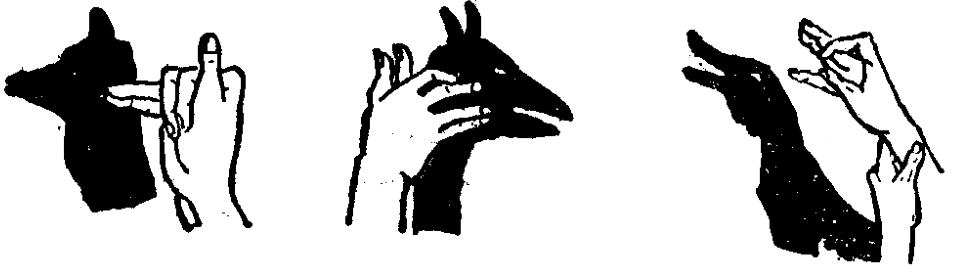
\includegraphics[width=0.7\textwidth]{../pic/czwl2-ch1-2}
    \caption{}\label{fig:1-2}
\end{figure}


(3) 在太阳光的照射下,人在地面上的影子为什么早晚长,中午短?画图来帮助说明。

(4) 天文学上常用光年〈就是光在一年内通过的距离)来做长度的单位,1 光年是多少千米?
织女星离地球约 27 光年,织女星离地球有多少千米?

(5) 有一位在北京某剧场里观看演出的观众坐在离演奏者 30 米远处,
另一位在上海的观众在自己家里电视机前看该剧场的电视转播演出,
北京与上海相距 1460 千米。问哪一位观众先听到演奏声?
电视是靠无线电波来转播的,而无线电波与光的传播速度相等。


\section*{小实验}

\begin{wrapfigure}[7]{r}{6cm}
    \centering
    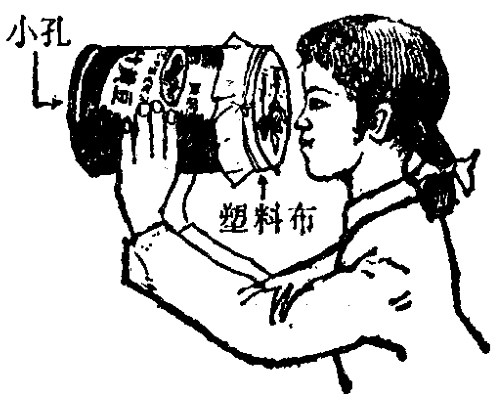
\includegraphics[width=4cm]{../pic/czwl2-ch1-3}
    \caption{}\label{fig:1-3}
\end{wrapfigure}

你可以自己做小孔成像的实验。找一个空罐头筒(或一个方纸盒)。
在筒底的中心用小铁钉开一个小孔(直径 1 毫米到 3 毫米),
在开口端蒙上一块半透明的塑料布(或纸)。
让罐头筒上的小孔对着房间外边明亮的景物,在你的头和罐头筒上面蒙上一件厚的深颜色衣服。
你在塑料布上就会看到一幅彩色的图像(图 \ref{fig:1-3}),只可惜是倒立的。

利用这样的装置,装上底片就可以拍摄出清晰的照片来。



\section{光的反射}\label{sec:1-2}

光射到物体表面上的时候,有一部分光会被物体表面反射回去。
这种现象叫做\textbf{光的反射}。 这一节我们就来研究光的反射。

光射到任何物体的表面,都会发生反射。我们选择对光反射能力强的平面镜来研究光的反射。
一束光照射到镜面被反射回去,可以看出,反射光仍然沿直线传播。
那么,反射光线的方向是由什么决定的呢?它跟照到镜面的入射光线有什么关系呢?
我们用如图 \ref{fig:1-4} 所示的装置来研究这个问题。

\begin{figure}[htbp]
    \centering
    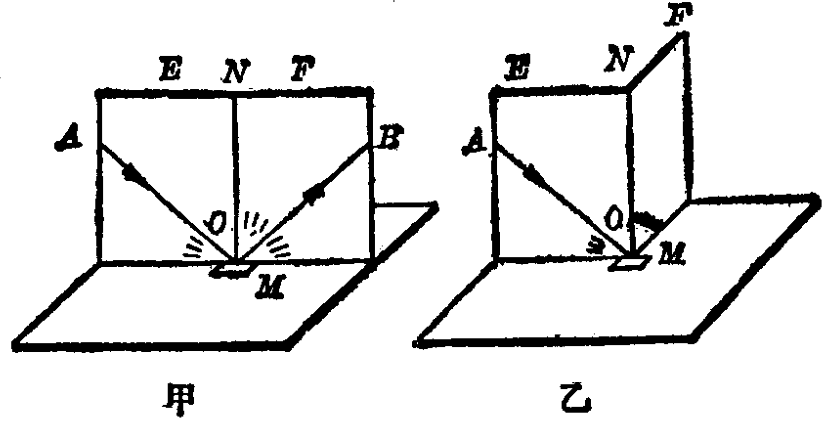
\includegraphics[width=0.7\textwidth]{../pic/czwl2-ch1-4}
    \caption{光的反射}\label{fig:1-4}
\end{figure}

$M$ 是平面镜,镶在一块木板上,在木板上立一块带有半圆刻度的白色屏,用来显示光束传播的路径。
这个屏是由两块长方形硬纸板 $E$、$F$ 粘连起来的,它们可以绕着接缝 $ON$ 向前折或者向后折。
把 $E$ 竖直地固定在木板上,然后让一束光沿 $E$ 上的 $AO$ 射到平面镜上的 $O$ 点。
转动 $F$,当它跟 $E$ 在同一平面时,就会在 $F$ 上看到有光束沿 $OB$ 射出(图 \ref{fig:1-4} 甲);
当 $F$ 在别的拉置时,就看不到反射光了(图 \ref{fig:1-4} 乙)。

我们把通过入射点 $O$ 垂直于镜面的直线 $ON$ 叫做\textbf{法线}。
从上面的实验可以看出,反射光线跟入射光线和法线在同一平面上。

在上面的实验里,还可以从屏上的圆形刻度盘上观察入射光线和反射光线的方向。
我们把入射光线 $AO$ 跟法线 $ON$ 的夹角 $\angle AON$ 叫做\textbf{入射角},
     反射光线 $OB$ 跟法线 $ON$ 的夹角 $\angle BON$ 叫做\textbf{反射角}。
让入射光线 $AO$ 沿不同的方向射入,观察反射光线 $OB$ 的方向,可以看出反射角总是等于入射角。

这样,我们就得到了光的\textbf{反射定律:
反射光线跟入射光线和法线在同一平面上,
反射光线和入射光线分居在法线的两侧;
反射角等于入射角}。

\begin{figure}[htbp]
    \centering
    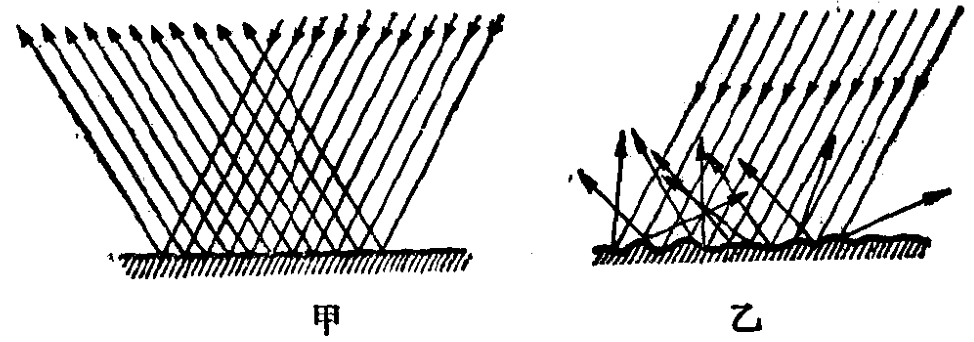
\includegraphics[width=0.7\textwidth]{../pic/czwl2-ch1-5}
    \caption{镜面反射(甲) 和漫反射(乙)}\label{fig:1-5}
\end{figure}

光射到任何表面上都会发生反射,但是从生活经验知道,不同的表面对光的反射是不一样的。
平滑的表面,例如镜面、抛光的金属面、平静的水面等;能使平行的入射光线沿着同一方向反射出去,
即反射光线也是平行的(图 \ref{fig:1-5} 甲)。
因此在这一方向上的反射光就强,而在其他方向上没有反射光。这种反射叫做\textbf{镜面反射}。
如果表面粗糙不平, 即使入射光线是平行的,反射后的光线也不平行,而是射向各个方向(图 \ref{fig:1-5} 乙)。
这种反射叫做\textbf{漫反射}。
必须注意,发生漫反射的时候,每一条光线还是遵守反射定律的。

一般物体的表面都是粗糙不平的。纸张、桌面、布等看起来是平的,可是仔细观察就知道都有些微小的凸凹不平。
光射到这些物体表面上的时候,就发生漫反射。
我们能从不同的方向看到这些本身不发光的物体,就是因为它们的表面能把射来的光向各个方向反射的缘故。


\section{平面镜成像}\label{sec:1-3}

\begin{wrapfigure}[11]{r}{5.5cm}
    \centering
    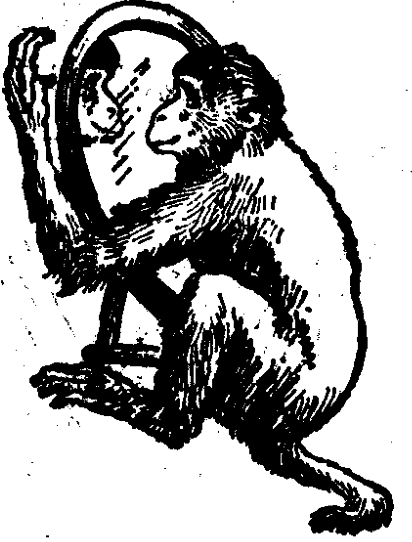
\includegraphics[width=4cm]{../pic/czwl2-ch1-6}
    \caption{}\label{fig:1-6}
\end{wrapfigure}


猴子从镜子里看到了一只猴子,想去镜后抓住它。结果什么也抓不着(图 \ref{fig:1-6})。
原来,聪明的猴子不懂得镜子里的猴子就是它自己的像。

日常生活里常用的镜子表面是平的,叫做\textbf{平面镜}。
这一节,我们就来研究平面镜成像。


在图 \ref{fig:1-7} 里,光从发光点 $S$ 发出,光线 $SA$、$SC$ 被镜面反射后,
分别沿 $AB$、$CD$ 的方向射进我们的眼睛里。
发光点虽然在 $S$,可是我们逆着反射光线的方向看去,
就觉得发光点好象在镜子后面的 $S_1$ 处,$S_1$ 就是发光点 $S$ 的像。
显然,实际上光线不是来自 $S_1$ 点,镜子后面也不存在发光点 $S_1$,所以这个像是\textbf{虚像}。

镜子前面的物体可以看成是由许多点组成的,每个点在镜子里都有一个像,这些像就组成物体的像。
物体在平面镜里的像也是虚像。

\begin{figure}[htbp]
    \centering
    \begin{minipage}{7cm}
    \centering
    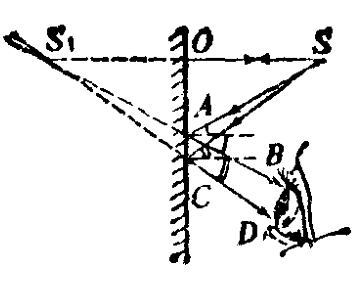
\includegraphics[width=4cm]{../pic/czwl2-ch1-7}
    \caption{}\label{fig:1-7}
    \end{minipage}
    \qquad
    \begin{minipage}{7cm}
    \centering
    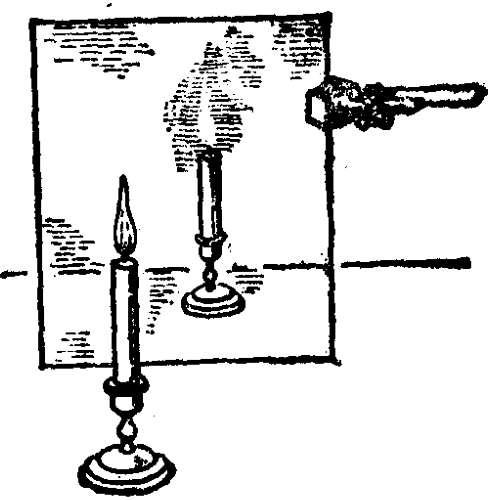
\includegraphics[width=5cm]{../pic/czwl2-ch1-8}
    \caption{}\label{fig:1-8}
    \end{minipage}
\end{figure}


在桌面上竖直地立一块玻璃板,玻璃板的前面点一支蜡烛(图 \ref{fig:1-8}),
就会看到玻璃板跟平面镜相似,在它的后面有蜡烛的像。
再拿一支同样的,不过没有点着的蜡烛,把它放在玻璃板的后面,
并且前后左右移动它,直到从玻璃前面的各处看来,这支蜡烛也好象点着似的为止。
这说明,没有点着的蜡烛恰好在点着的蜡烛的虚像的位置上,而且它们的大小相等;
如果测量下,还会发现,两支蜡烛的连线跟玻璃板垂直,它们到玻璃板的距离相等。

可见,\textbf{物体在平面镜里成的是虚像;像和物体的大小相等,
它们的连线跟镜面垂直,它们到镜面的距离相等}。

光滑的金属面,平静的水面,都具有平面镜的作用,能够形成清晰的像。
在玻璃发明以前,古代的人就用磨光的铜盘做镜子。
平静的水面能够清楚地映出岸上的景物,造成美丽的景色(\hyperref[fig:pic1]{彩图1}), 也是平面镜成像的结果。

\begin{figure}[htbp]
    \centering
    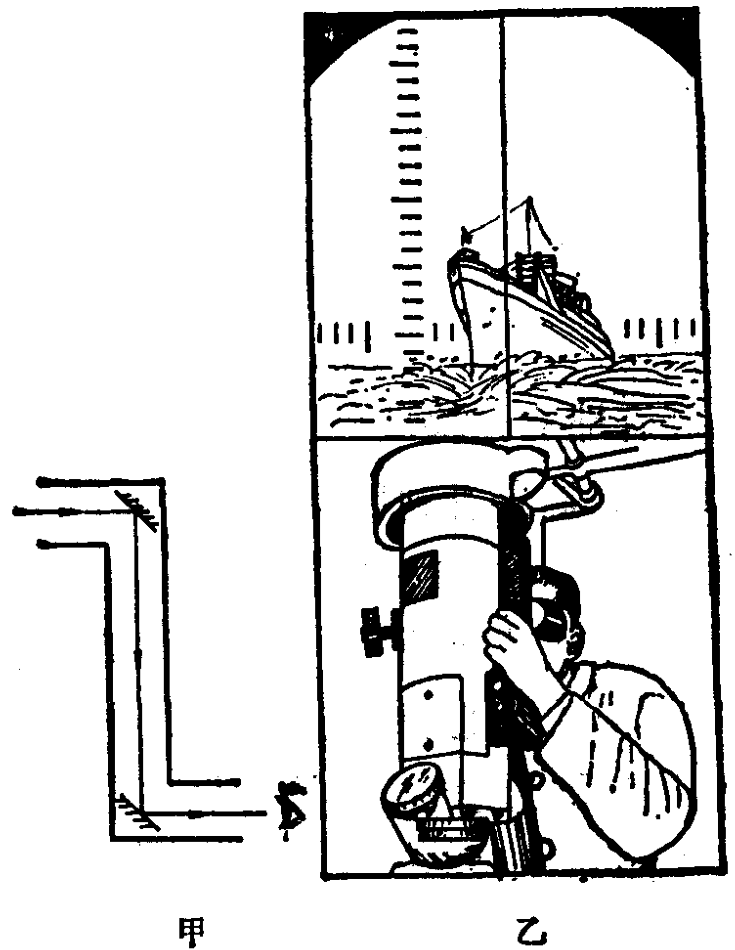
\includegraphics[width=0.6\textwidth]{../pic/czwl2-ch1-9}
    \caption{潜望镜}\label{fig:1-9}
\end{figure}

平面镜还广泛安装在各种仪器中,用来改变光线的方向。
潜望镜就是其中的一个例子,最简单的潜望镜(图 \ref{fig:1-9} 甲)是在管子的上方和下方拐角处各装一块平面镜,
两块平面镜互相平行,都跟水平方向成 $45^\circ$ 角。
高处物体沿水平方向射入镜筒中的光线经两块平面镜反射后仍沿水平方向射出,进入观察者的眼中。
这样就可以从潜望镜中看见被掩蔽物挡住的物体。
潜望镜可以用在战壕里,潜水艇里,观察外面的情况(图 \ref{fig:1-9} 乙)。

平面镜成像的现象有时对我们不利。
例如,汽车在夜间行驶的时候,假如车内开着灯,司机前面的玻璃窗就会象平面镜那样,
反射车内物体投射来的光,使司机看见车内物体的像,而妨碍看清前面的道路。
因此,汽车在夜间行驶,车内不开灯,以保证行车安全。


\section{球面镜}\label{sec:1-4}

实际上还常常用到\textbf{球面镜},它的反射面是球面的一部分。球面镜有两种,
  一种是用球面的里面做反射面的,叫做\textbf{凹镜};
另一种是用球面的外面做反射面的,叫做\textbf{凸镜}。

把凹镜对着太阳,太阳的平行光被凹镜反射后,就会聚在一点 $F$(图 \ref{fig:1-10})。
如果把一块小纸片放在这一点,小纸片上就出现一个明亮的点。过一会儿,
亮点处的纸就被烧焦。这一点就叫做凹镜的\textbf{焦点}。

利用凹镜能把太阳光会聚在焦点的性质,可以制成煮饭、烧水用的太阳灶和给蒸汽轮机
生产水蒸气或者熔化难熔物质的太阳炉。需要加热的物体就放在凹镜的焦点处。
凹镜的面积越大,能够会聚的太阳光就越多,焦点处的温度就越高。
\hyperref[fig:pic2]{彩图2} 所示的是太阳能焊接机。
它的凹镜的直径为 2.5 米,焦点处的温度可达 $2000\celsius$,能使金属熔化,进行焊接。

\begin{figure}[htbp]
    \centering
    \begin{minipage}{7cm}
    \centering
    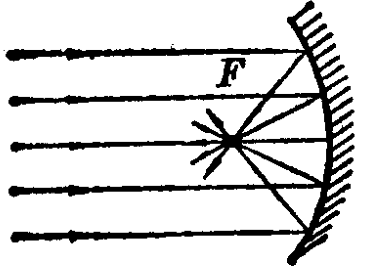
\includegraphics[width=5cm]{../pic/czwl2-ch1-10}
    \caption{凹镜能使平行光\\会聚在焦点上}\label{fig:1-10}
    \end{minipage}
    \qquad
    \begin{minipage}{7cm}
    \centering
    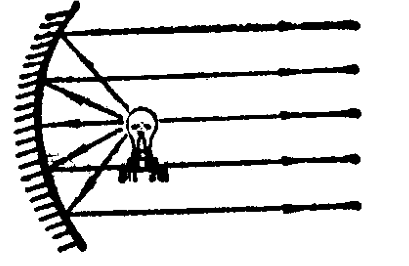
\includegraphics[width=5cm]{../pic/czwl2-ch1-11}
    \caption{从凹镜焦点发出的光\\被反射后平行射出}\label{fig:1-11}
    \end{minipage}
\end{figure}


如果把光源放在凹镜的焦点上,光源发出的光被凹镜反射以后,将成为平行光(图 \ref{fig:1-11})。
汽车头灯(图 \ref{fig:1-12})就是利用凹镜的这种性质做成的。汽车头灯是双光灯,它有两个灯丝:
一个是远距光灯丝,在凹镜的焦点上,发出的光经凹镜反射后集中向前方平行射出,照亮远处的道路;
另一个是近距光灯丝,不在凹镜的焦点上,发出的光经凹镜反射后只照亮车前不远的地方,
可以避免使对面开来的汽车司机感到刺眼。

\begin{figure}[htbp]
    \centering
    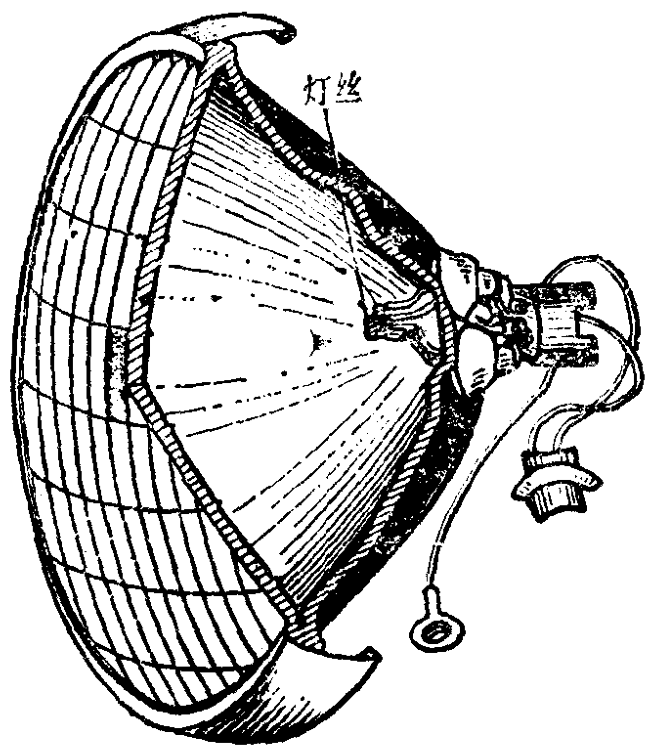
\includegraphics[width=0.5\textwidth]{../pic/czwl2-ch1-12}
    \caption{汽车头灯}\label{fig:1-12}
\end{figure}


凸镜对于光起发散作用。射到凸镜上的平行光,经凸镜反射后不能会聚于一点,而是变得发散(图 \ref{fig:1-13})。

\begin{figure}[htbp]
    \centering
    \begin{minipage}{7cm}
    \centering
    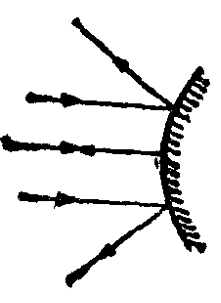
\includegraphics[width=4cm]{../pic/czwl2-ch1-13}
    \caption{凸镜能使平行光发散}\label{fig:1-13}
    \end{minipage}
    \qquad
    \begin{minipage}{7cm}
    \centering
    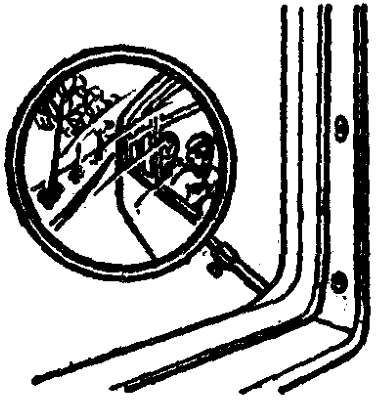
\includegraphics[width=6cm]{../pic/czwl2-ch1-14}
    \caption{汽车上的观后镜}\label{fig:1-14}
    \end{minipage}
\end{figure}

汽车驾驶室外面的观后镜常用凸镜(图 \ref{fig:1-14})。为什么用凸镜而不用平面镜呢?
从图 \ref{fig:1-15} 中可以看出,对于口径相同的平面镜和凸镜来说,当人离镜同样远时,
从凸镜观察到的范围要比平面镜大。
\begin{figure}[htbp]
    \centering
    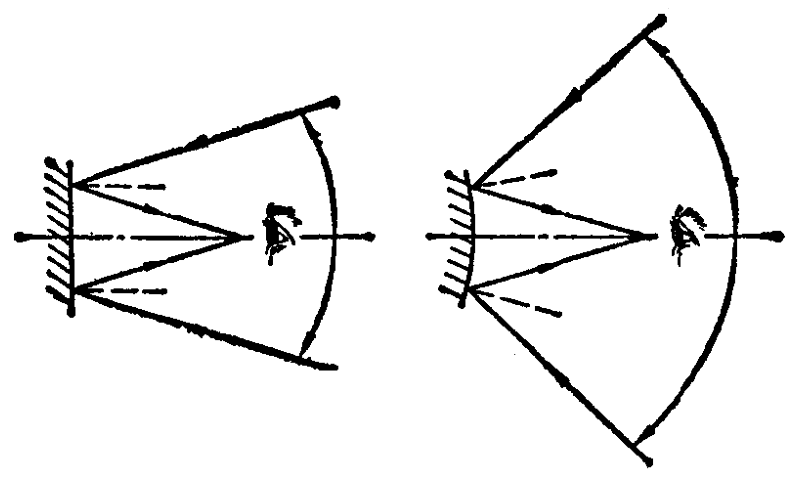
\includegraphics[width=0.6\textwidth]{../pic/czwl2-ch1-15}
    \caption{}\label{fig:1-15}
\end{figure}
汽车上用凸镜做观后镜,可以使司机从镜中观察到车后侧较大范围内的物体,保证行车安全。
有的城市在马路交叉处和拐弯处也常常安装一个大的凸镜,
使交通民警和行人以看到较大范围的车辆行驶情况,保证交通安全。


\lianxi

(1) 入射光线跟镜面的夹角是 $25^\circ$,入射光线跟反射光线的夹角是多少?

(2) 要想使反射光线跟入射光线成直角,入射角应当是多大?
如果使入射光线逐渐靠拢法线,反射光线的方向怎样变化?

(3) 在黑喑的房子里,桌子上立着一平面镜,镜子后面是白色的墙。
用手电筒正对着镜子和墙照射,从旁边看时,会发现墙被照亮了,而镜子却显得很暗〈图 \ref{fig:1-16})。
实际做做看,并说明为什么墙反而比镜子亮。

\begin{figure}[htbp]
    \centering
    \begin{minipage}{7cm}
    \centering
    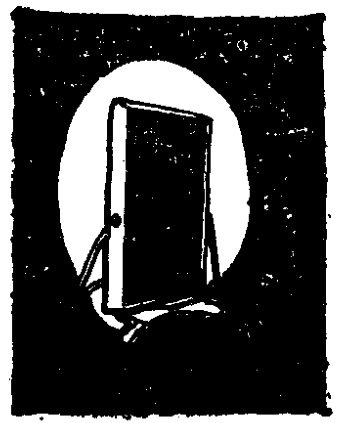
\includegraphics[width=5cm]{../pic/czwl2-ch1-16}
    \caption{}\label{fig:1-16}
    \end{minipage}
    \qquad
    \begin{minipage}{7cm}
    \centering
    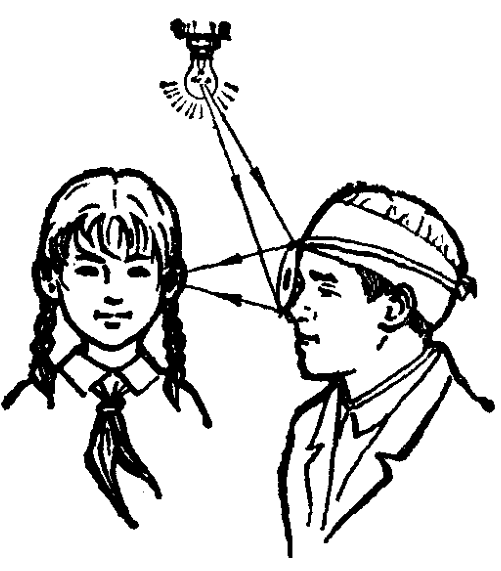
\includegraphics[width=5cm]{../pic/czwl2-ch1-17}
    \caption{}\label{fig:1-17}
    \end{minipage}
\end{figure}

(4) 一人立于平面镜前 1 米处,这个人在镜子里的像离他本人多远?
如果人向镜面前进 0.5 米,人和像间的距离又是多少?

(5) 医生检查耳道时,为什么常戴一个凹镜(图 \ref{fig:1-17})。



\section{光的折射}\label{sec:1-5}

在第一节里已经说过,光从一种物质进入另一种物质,它的传播方向通常会改变。
这种现象叫做光的\textbf{折射}。现在用实验来研究光的折射。

\begin{wrapfigure}[13]{r}{7cm}
    \centering
    %\includegraphics[width=7cm]{../pic/czwl2-ch1-18}
    \begin{tikzpicture}[>=Stealth, scale=0.9]
    \draw (-3, 0) -- (3, 0);
    \draw [dashed] (0, 3) -- (0, -3);
    \node at (3.7, 0) {分界面};
    \node at (-2.6, 0.4) {空气};
    \node at (-2.6, -0.4) {水};
    \node at (0.3, -0.3) {$O$};
    \node at (0.4, 2.7) {$N$};
    \node at (0.4, -2.7) {$N'$};

    \draw [rotate=50] (0, 0) -- (3, 0) [->] (2, 0) -- (1, 0);
    \draw (0, 0.8) arc [start angle=90, end angle=50, radius=0.8];
    \draw (0, 0.7) arc [start angle=90, end angle=50, radius=0.7];
    \node at (1.2, 2.0) {$A$};
    \node at (2.2, 1.5) {入射光};

    \draw [rotate=-50] (0, 0) -- (-3, 0) [->] (0, 0) -- (-1.2, 0);
    \draw (0, 0.75) arc [start angle=90, end angle=130, radius=0.75];
    \draw (0, 0.65) arc [start angle=90, end angle=130, radius=0.65];
    \node at (-2.2, 1.5) {反射光};

    \draw [rotate=60] (0, 0) -- (-3, 0) [->] (0, 0) -- (-1, 0);
    \draw (0, -0.65) arc [start angle=270, end angle=240, radius=0.65];
    \node at (-1.1, -2.4) {$B$};
    \node at (-1.9, -1.7) {折射光};
\end{tikzpicture}

    \caption{光的折射}\label{fig:1-18}
\end{wrapfigure}

让一束光从空气斜着射向水面,我们会看到,除了有一部分光反射回空气,改变了传播方向以外,
还有一部分光进入水中,也改变了传播方向(图 \ref{fig:1-18})\footnotemark。
\footnotetext{注:原书的图模糊不清,我使用 tikz 绘制了一个图片。} % 原书图片 保存为 pic 目录下的 czwl2-ch1-18.old.png

在图 \ref{fig:1-18} 里,法线是直线 $NN'$,入射角是 $\angle AON$。
折射光线 $OB$ 跟法线的夹角 $\angle BON'$ 叫做\textbf{折射角}。

在上面的实验里,如果增大或减小入射角,折射角就随着增大或减小。
但是,只要光是从空气斜射入水里,就会发生折射,并且折射角总小于入射角。

当光从水斜射入空气里的时候,也发生折射,例如光沿图 \ref{fig:1-18} 里 $BO$ 的方向从水里射到分界面上,
它就沿着 $OA$ 的方向折射。这时候折射角大于入射角。

不论光是从空气射入水里, 还是从水射入空气里,如果光是沿着法线方向入射的,通过分界面以后,
光的传播方向不改变。

从实验还可以看出,折射光线总是跟入射光线和法线在同一平面上。

如果换用别的透明物质代替水来做上面的实验,可以得到同样的结果,因此我们得到下面的结论:

\textbf{折射光线跟入射光线和法线在同一平面上,折射光线和入射光线分居在法线的两侧}。

\textbf{%
光从空气斜射入水或别的透明物质里时,折射角小于入射角;
光从水或别的透明物质斜射入空气里时,折射角大于入射角}。

在日常生活中,可以看到许多光的折射现象。
例如,插入水中的筷子,水里的部分,从水面上斜着看起来向上折了(图 \ref{fig:1-19}),就是由于光的折射的缘故。
从筷子下端 $B$ 点射出的光由水中进入空气中时,在水面处发生折射,远离法线,折射光射入眼里,
人的视觉就觉得折射光是从它的反方向延长线的 $B'$ 点发出的,$B'$ 就是 $B$ 的像。
筷子浸在水中的一段 $AB$ 上其他各点情形也是这样。因此我们就觉得整个 $AB$ 段向上折了。

\begin{figure}[htbp]
    \centering
    \begin{minipage}{7cm}
    \centering
    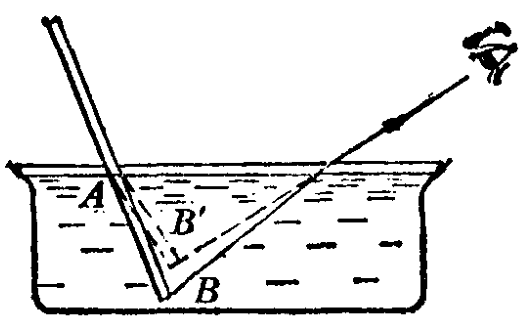
\includegraphics[width=7cm]{../pic/czwl2-ch1-19}
    \caption{插入水中的筷子变得向上弯折}\label{fig:1-19}
    \end{minipage}
    \qquad
    \begin{minipage}{7cm}
    \centering
    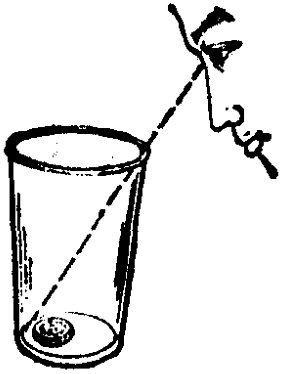
\includegraphics[width=4cm]{../pic/czwl2-ch1-20}
    \caption{}\label{fig:1-20}
    \end{minipage}
\end{figure}


\section*{小实验}

在空的茶杯里放一枚分币,移动怀子,使眼睛刚刚看不到分币(图 \ref{fig:1-20})。
保持眼睛和杯子的位置不变,慢慢地向杯里倒水。随着水面的升高,你会看到什么现象?
根据光的折射知识,对你的实验作出解释。



\section{透镜}\label{sec:1-6}

透镜是照相机、幻灯机等光学仪器的重要组成部分,通常是用玻璃磨成的。
它的一个侧面,或者两个侧面是球面的一部分。透镜可以分成两类:
一类是中央比边缘厚的,叫做\textbf{凸透镜},象图 \ref{fig:1-21} 里的 1、2、3;
另一类是中央比边缘薄的,叫做\textbf{凹透镜},象图 \ref{fig:1-21} 里的 4、5、6。

\begin{figure}[htbp]
    \centering
    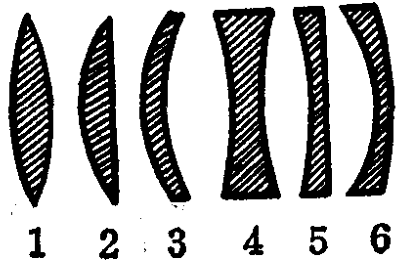
\includegraphics[width=0.3\textwidth]{../pic/czwl2-ch1-21}
    \caption{各种透镜}\label{fig:1-21}
\end{figure}

让一束平行光射在凸透镜上(图 \ref{fig:1-22}),可以看到,光通过凸透镜发生折射以后会聚于一点,
可见凸透镜对光有会聚作用,所以又叫做\textbf{会聚透镜}。

\begin{figure}[htbp]
    \centering
    \begin{minipage}{7cm}
    \centering
    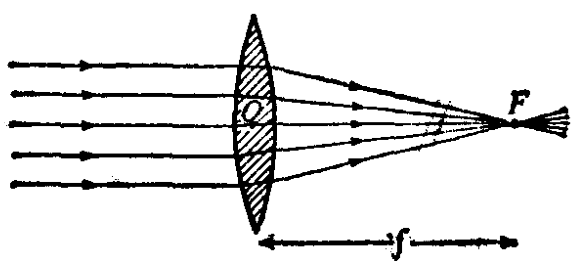
\includegraphics[width=6.5cm]{../pic/czwl2-ch1-22}
    \caption{凸透镜的会聚作用}\label{fig:1-22}
    \end{minipage}
    \qquad
    \begin{minipage}{7cm}
    \centering
    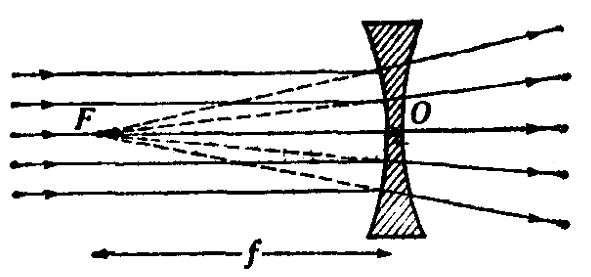
\includegraphics[width=6.5cm]{../pic/czwl2-ch1-23}
    \caption{凹透镜的发散作用}\label{fig:1-23}
    \end{minipage}
\end{figure}

让一束平行光射在凹透镜上(图 \ref{fig:1-23}),可以看到,光通过凹透镜发生折射以后向外散开。
可见凹透镜对光有发散作用,所以又叫做\textbf{发散透镜}。

\begin{figure}[htbp]
    \centering
    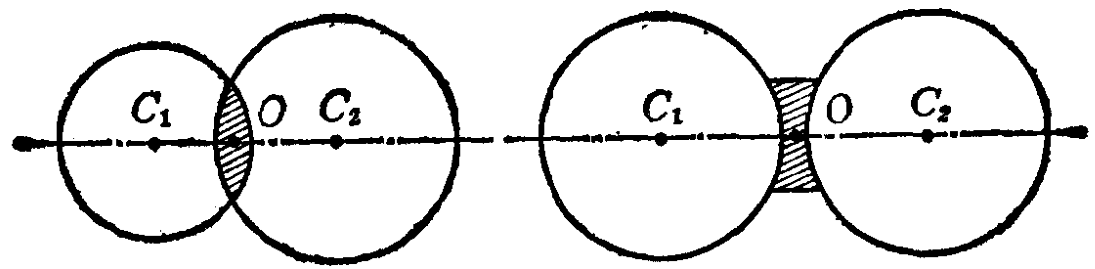
\includegraphics[width=0.7\textwidth]{../pic/czwl2-ch1-24}
    \caption{透镜的主轴}\label{fig:1-24}
\end{figure}

通过透镜两个球面的球心 $C_1$、$C_2$ 的直线,叫做透镜的\textbf{主轴}(图 \ref{fig:1-24})。
如果透镜的一个侧面是平面,透镜的主轴就跟这个平面垂直,并且通过另一侧面的球心。
通常用的透镜,厚度比球面的半径小得多,叫薄透镜。在中学里只研究薄透镜。

跟主轴平行的光通过凸透镜后会聚在主轴上的一点(图 \ref{fig:1-22} 中的 $F$),这个点叫做凸透镜的\textbf{焦点}。
跟主轴平行的光通过凹透镜后形成一个发散的圆锥(图 \ref{fig:1-23}),这些发散的光,
看起来象是从它们传播方向的反向延长线的交点 $F$ 发出来的,点 $F$ 也在主轴上,叫做凹透镜的焦点。
可见凹透镜的焦点不是光实际会聚点,所以是虚焦点,而凸透镜的焦点是光实际会聚点,所以是实焦点。
焦点到透镜中心 $O$ 的距离叫做\textbf{焦距},通常用 $f$ 表示。
透镜的两侧各有一个焦点,两个焦点到中心的距离相等。

\begin{wrapfigure}[11]{r}{7cm}
    \centering
    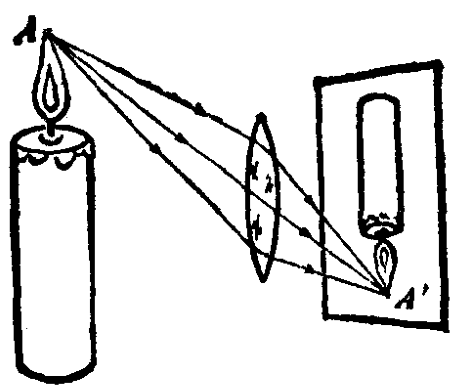
\includegraphics[width=6cm]{../pic/czwl2-ch1-25}
    \caption{光的折射}\label{fig:1-25}
\end{wrapfigure}

实验表明,如果把光源放在凸透镜的焦点上,光源发出的光通过凸透镜后一定平行射出。

凸透镜不但对光有会聚作用,而且还能够成像。

如图 \ref{fig:1-25} 所示,把凸透镜放在蜡烛和光屏的中间,调整它们的位置,可以在光屏上得到蜡烛的倒立像。
这个像是怎样形成的呢?我们先来考察顶端的一点 $A$。这一点发出的光向四周散射,其中一部分射到凸透镜上,
通过凸透镜的光线发生折射会聚于一点 $A'$,点 $A'$ 就是点 $A$ 的像。
同样,蜡烛上的每一点都产生一个像点。这许多像点组成了整个蜡烛的像。
这里,凸透镜所成的像是通过凸透镜的光实际会聚而成的,叫做\textbf{实像}。



\section{实验:研究凸透镜成像}\label{sec:1-7}

凸透镜能够使物体成像,物体离凸透镜的距离不同,所成的像也不同。
我们做实验来研究凸透镜成像的各种情况。

实验可以在如图 \ref{fig:1-26} 所示的光具座上进行。用蜡烛火焰作为物体,
研究它发出的光通过焦距已知的凸透镜后在光屏上所成的像。

\begin{figure}[htbp]
    \centering
    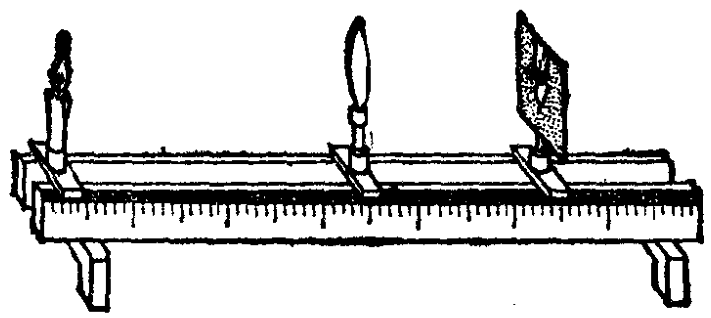
\includegraphics[width=0.7\textwidth]{../pic/czwl2-ch1-26}
    \caption{}\label{fig:1-26}
\end{figure}

在光具座上由左向右依次放置蜡烛、凸透镜和光屏。为了使烛焰的像能成在光屏的中间,
要调整凸透镜和光屏的高度,使它们的中心跟烛焰的中心大致在同一高度。

先调整凸透镜的位置,使蜡烛到凸透镜的距离(简称为物距,用 $u$ 来表示)大于凸透镜焦距的二倍(即 $u > 2f$)。

沿光具座移动光屏,直到光屏上出现清晰的烛焰像为止。
观察光屏上的像是倒立的还是正立的,是放大的还是缩小的。
测出像到凸透镜的距离(简称为像距,用 $v$ 来表示),把这时的像距跟焦距、二倍焦距相比较。
把观察和测量、比较的结果填入下面的表里。

\begin{tblr}{
    hlines, vlines, stretch=1.3,
    colspec={Q[c,8em]ccQ[c,8em]},
    cells={valign=m},
}
    \SetCell[r=2]{c}{物距 \\ ($u$)} & \SetCell[c=2]{c}{像的性质} & & \SetCell[r=2]{c}{像距 \\ ($v$)} \\
    & 倒立或成立 & 放大或缩小 & \\
    $u > 2f$ & & & \\
    $2f > u >f$ & & & \\
\end{tblr}

再向左移动凸透镜的位置,减小物距,使蜡烛位于二倍焦距与焦点间($2f > u >f$),照上一段要求的那样,
移动光屏,在光屏上得到清晰的烛焰像,进行观察和测量、比较,把结果填入上面表里。

蜡烛位于焦点以外,物距不断减小的过程中,像距怎样变?像的大小怎样变?

如果继续向左移动凸透镜的位置,使蜡烛位于焦点以内($u < f$),移动光屏,在光屏上能不能得到烛焰像?
从光屏这一侧透过凸透镜观察烛焰,能看到一个正立、放大的烛焰像吗?


\section{凸透镜的应用}\label{sec:1-8}

\xiaobiaoti{凸透镜成像的几种情况}
从上一节的实验,我们可以得到如图 \ref{fig:1-27} 所示的凸透镜成像的情况。

\begin{figure}[H]
    \centering
    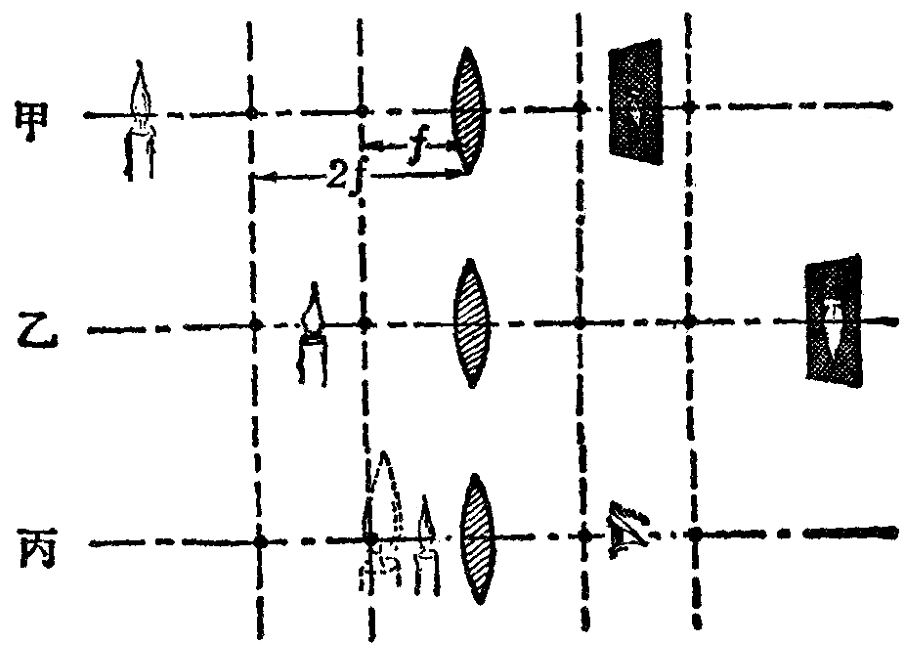
\includegraphics[width=0.6\textwidth]{../pic/czwl2-ch1-27}
    \caption{凸透镜成像}\label{fig:1-27}
\end{figure}

物体在凸透镜的焦点以外的时候,在透镜另一侧的光屏上总能得到倒立的实像,并且物距越小,像就越大,像距也越大。
当 $u > 2f$ 时,像是缩小的,$f < v < 2f$ (图 \ref{fig:1-27} 甲);
当 $2f > u > f$ 时,像是放大的,$v > 2f$(图 \ref{fig:1-27} 乙)。

物体在凸透镜的焦点以内的时候,在透镜的另一侧得不到物体的实像,
透过透镜可以看到正立、放大的像(图 \ref{fig:1-27} 丙)。
这个像跟平面镜成像相似,不是物体上各点发出的光实际会聚成的,所以是虚像。

\xiaobiaoti{照相机} 当 $u > 2f$ 时,凸透镜能够成缩小的实像,照相机就是利用这种现象来拍摄照片的。

\begin{figure}[htbp]
    \centering
    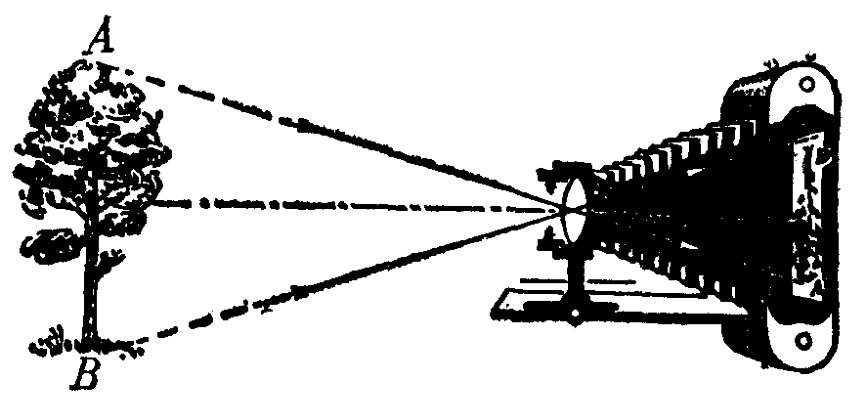
\includegraphics[width=0.6\textwidth]{../pic/czwl2-ch1-28}
    \caption{照相机示意图}\label{fig:1-28}
\end{figure}

照相机(图 \ref{fig:1-28})的前部有一个镜头,通常是由一组透镜组成的,它的作用相当于一个凸透镜。
镜头后面是暗箱,照相的感光胶片就装在暗箱的底部。选定了被照景物和照相的位置后,
调节暗箱的长度,也就是调节镜头的位置,使胶片上得到被照景物的清晰的倒立、缩小的实像。
胶片上的感光物质受到形成实像的光的照射,发生了化学变化,经过处理就得到底片,
然后由底片就可以得到照片。


\xiaobiaoti{幻灯机} 当 $2f > u > f$ 时,凸透镜能够成放大的实像,幻灯机就是利用这种现象,
把幻灯片上景物的像投射到银幕上的。

\begin{figure}[htbp]
    \centering
    \begin{minipage}{9cm}
    \centering
    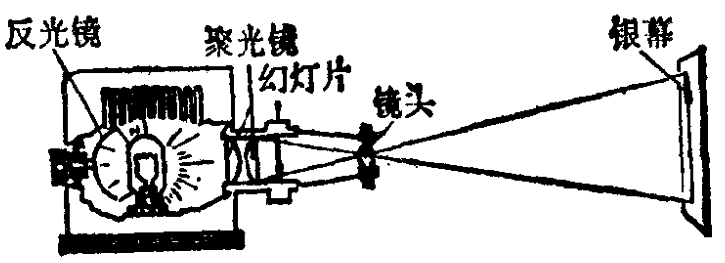
\includegraphics[width=8.5cm]{../pic/czwl2-ch1-29}
    \caption{幻灯机示意图}\label{fig:1-29}
    \end{minipage}
    \qquad
    \begin{minipage}{6cm}
    \centering
    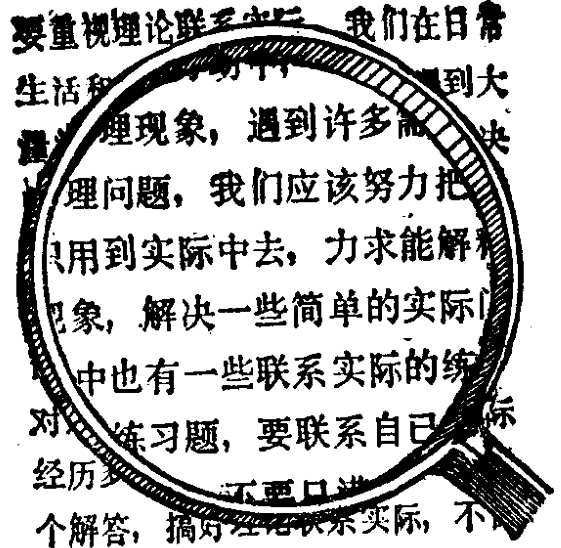
\includegraphics[width=4cm]{../pic/czwl2-ch1-30}
    \caption{放大镜}\label{fig:1-30}
    \end{minipage}
\end{figure}


图 \ref{fig:1-29} 是幻灯机的示意图。它前部的镜头相当于一个凸透镜,透明的幻灯片插在凸透镜后面比焦点略微远些的地方。
幻灯片后面是聚光镜,再后面是很强的光源和反光镜。光源发出的光和反光镜反射的光,经过聚光镜强烈地照亮幻灯片,
前后调整镜头的位置,银幕上就会出现幻灯片上景物的倒立、放大的实像。
我们要看到正立的像,只要把幻灯片倒过来插就行了。

\xiaobiaoti{放大镜} 当 $u < f$ 时,凸透镜能够成放大的虚像,放大镜就是利用这种现象来观察物体的。

使用放大镜的时候,必须把要观察的物体放在焦点以内才能看到正立、放大的虚像(图 \ref{fig:1-30})。



\section*{阅读材料:电影}

\begin{wrapfigure}[29]{r}{6.5cm}
    \centering
    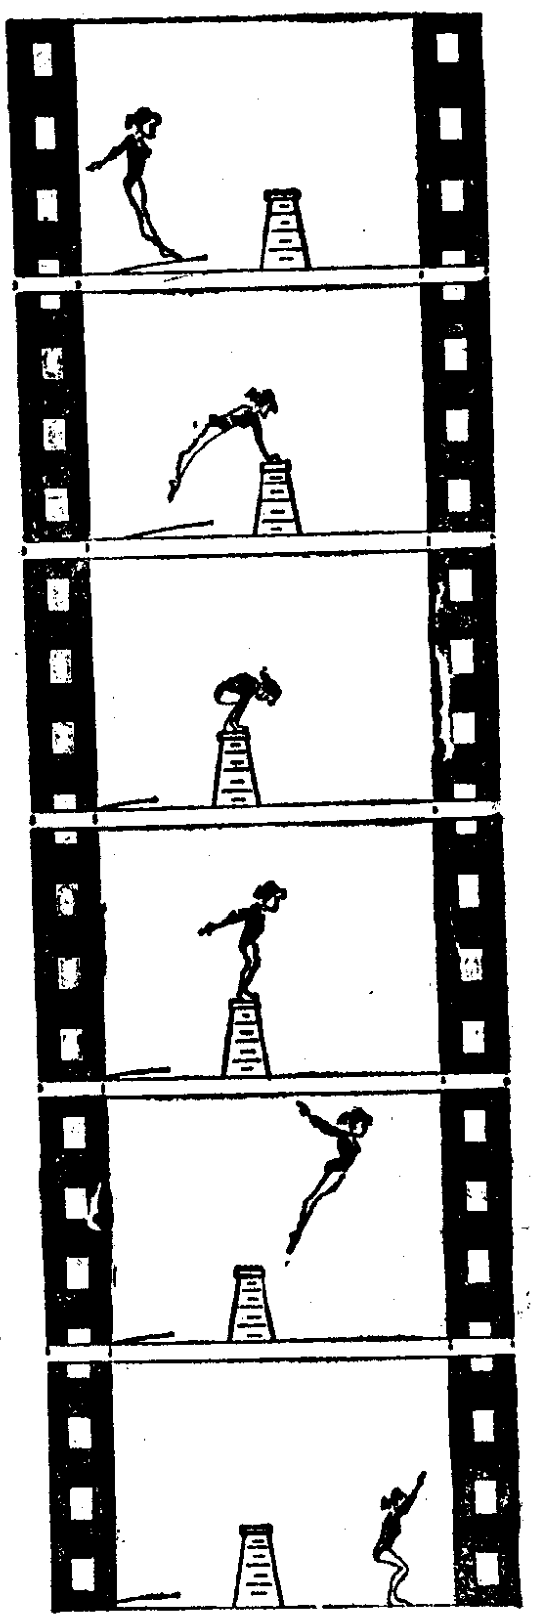
\includegraphics[width=5.5cm]{../pic/czwl2-ch1-31}
    \caption{电影片}\label{fig:1-31}
\end{wrapfigure}


电影放映机的构造相当复杂,但是它的投影原理跟幻灯机差不多,
也是利用相当于凸透镜的镜头把电影片上景物的像射到银幕上的。
不同的是,电影的画面是活动的。

\begin{enhancedline}
电影片上有一连串的照片。这些照片是对活动的景物每隔了 $\dfrac{1}{24}$ 秒拍一张拍摄下来的,
也就是说,一秒钟内要依次拍摄 24 张照片。因此,后一张跟前一张的景物的变化相差很小。
例如,拍摄体操运动员 6 ~ 7 秒钟内完的一个动作,在电影片上就留下了一百多张连续的照片。
图 \ref{fig:1-31} 是从这个过程中选出来的几个画面。
放映时,用电动机带动电影片,使它上面的照片依次从镜头后面通过,每秒钟通过 24 张。
每张照片都要在镜头后面停顿大约 0.04 秒的时间,它的放大的实像也在银幕上停留相同的时间。
在换照片的时候,电影放映机上有一个特殊的装置把镜头遮住,使银幕暂时黑暗。
但是我们看电影的时候,却觉得银幕上总有像,并且像中的景物是连续活动的,这是为什么呢?
\end{enhancedline}

这是因为人的视觉有一种叫做视觉暂留的特性,就是外界的景物消失以后,视神经对它的印象还会保留 0.1 秒的时间。
在黑暗中,迅速地移动一支点燃着的香,会看到香的亮点变成了一条亮线,就是由于视觉暂留。
放电影时,银幕上相继出现的像相隔的时间(也就是银幕黑暗的时间)不到 0.01 秒,并且它们上面的景物变化很小,
由于视觉暂留的缘故,我们就觉得像是连续活动的了。

通常,我们看的电影,银幕上的景物活动的情况跟实际上的快慢程度是一致的。
这是因为拍摄电影跟放映电影的速度相同,即拍摄时每秒拍 24 张,放映时也是每秒放 24 张。
如果拍摄时加快拍摄速度,例如每秒拍 3900 张,而放映时仍每秒放 24 张,那么银幕上的动作就会比实际的慢一百六十多倍。
实际的动作在电影里就是慢悠悠的了。这就是电影里的慢镜头。
相反,如果放慢拍摄速度,而按正常速度放映,结果银幕上的动作就会比实际的快。
实际的动作是很缓慢的,在电影里却是刹那间完成了。这就是电影里的快镜头。

电影的快、慢镜头,不但在一般的电影里被用来达到一定的艺术效果,在科学研究上也很重要。
例如,使用慢镜头可以更仔细地观察一个物体的运动。

电影不但丰富了我们的文化生活,而且能能够把各种活动情况有声有色地记录下来。
因此,电影是一种很好的记录工具。



\lianxi

(1) 有经验的渔民在叉鱼的时候,不把叉对准所看到的鱼的位置,而是对着稍低于所看到的鱼的位置叉去,才能叉到鱼。为什么?

(2) 图 \ref{fig:1-32} 中画出了光通过透镜前后的方向,在图中填上适当类型的透镜。

\begin{figure}[htbp]
    \centering
    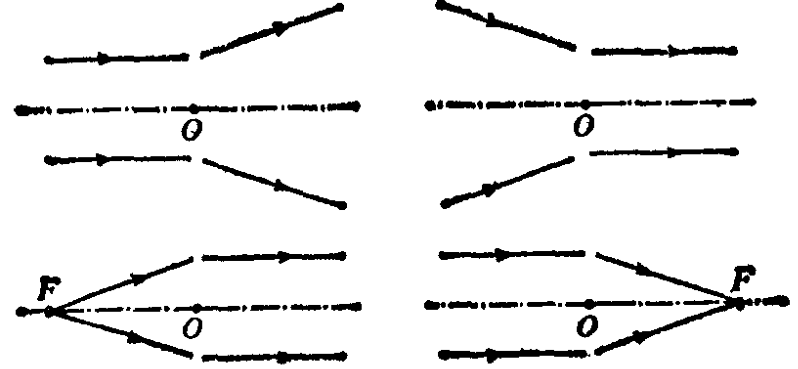
\includegraphics[width=0.6\textwidth]{../pic/czwl2-ch1-32}
    \caption{}\label{fig:1-32}
\end{figure}

(3) 有两个凸透镜,要想使一束跟它们的主轴平行的光通过它们后仍平行射出,这两个凸透镜应当怎样放置?
画出这一束光通过这两个凸透镜的情况。

(4) 用镜头焦距一定的照相机照相,想使照片上的人像大一些,照相机应该离被照的人近一些,还是远一些?

(5) 放映幻灯的时候,想使银幕上的像大一些,应该使幻灯机离银幕近一些,还是远一些?


\section{光的色散}\label{sec:1-9}

取一个棱镜,照图 \ref{fig:1-33} 那样,让一束白光(例如太阳光)穿过狭缝射在棱镜上。
可以看到,白光通过棱镜以后不但改变了方向,而且在白纸屏上形成一条彩色的光带。
\begin{figure}[htbp]
    \centering
    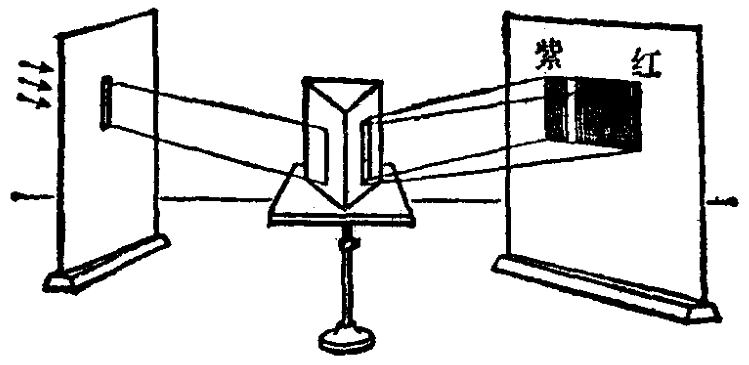
\includegraphics[width=0.6\textwidth]{../pic/czwl2-ch1-33}
    \caption{白光的色散}\label{fig:1-33}
\end{figure}
这条彩色光带上的颜色,从一端到另一端依次是红、橙、黄、绿、蓝、靛、紫。
这表明白光通过棱镜以后分解成各种色光。

\begin{figure}[htbp]
    \centering
    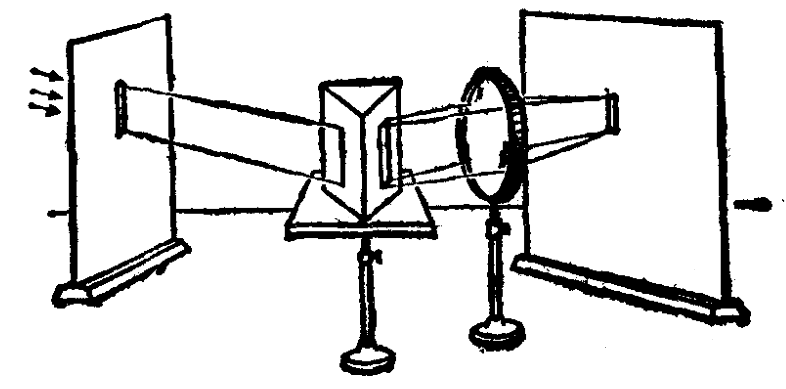
\includegraphics[width=0.6\textwidth]{../pic/czwl2-ch1-34}
    \caption{}\label{fig:1-34}
\end{figure}

如果照图 \ref{fig:1-34} 那样,把一个凸透镜放在棱镜和白纸屏之间,使这些色光会聚在纸屏上,
纸屏上就会出现一条白色光带。这表明色光合在一起又成了白色。

在图 \ref{fig:1-33} 的实验里,假如在纸屏上开一条狭缝,使彩色光带中的某种色光通过它,
再射到第二个棱镜上,那么这种色光通过第二个棱镜以后,就只改变方向,而不再分解成其他的色光了。

从上面的实验知道,白光是由各种色光混合而成的,白光通过棱镜以后,
分解成的各种色光是具有单纯颜色的光,不能再分解成其他的色光。

不能再分解的色光叫做\textbf{单色光},
由单色光混合成的光叫做\textbf{复色光}。
复色光分解成单色光的现象,叫做光的\textbf{色散}。



\section{物体的颜色}\label{sec:1-10}

了解了光的色散,就可以进一步研究物体为什么有各种各样的颜色。

在图 \ref{fig:1-33} 所示的实验里,在棱镜和白纸屏之间,
如果放一块红玻璃,屏上就只出现一条红光带,
如果放一块蓝玻璃,屏上就只出现一条蓝光带。
这个实验表明,某种颜色的透明体所透过的主要是同种颜色的色光,而其他的色光几乎都被吸收了。

所以,\CJKunderwave{透明体的颜色是由它透过的色光决定的}。

透明体如果几乎让各种色光都全部透过,它就是无色的。
空气、玻璃和洁净的水,都是常见的无色透明体。

在图 \ref{fig:1-33} 的实验里,在白纸屏上
如果贴上一张红纸,屏上就只有被红光照射的部分是亮的,
如果贴  一张蓝纸,屏上就只有被蓝光照射的部分是亮的。
这个实验表明,某种颜色的不透明体所反射的主要是同种颜色的色光,而其他的色光几乎都被吸收了。

所以,\CJKunderwave{不透明体的颜色是由它反射的色光决定的}。

不透明体
如果几乎使各种色光都全部反射,它就是白色的,
如果几乎把各种色光都全部吸收,它就是黑色的。

把两种颜色不同的颜料混合在一起,可以得到另外一种颜色。这是什么缘故呢?

每一种颜色的颜料,除了反射跟它相同的色光以外,还反射一些别种色光,不过比较弱。例如
黄颜料除了反射黄光,还反射橙光和绿光,
蓝颜料除了反射蓝光,还反射绿光和靛光。
如果黄、蓝这两种颜料混合在一起,能反射的就只有绿光了,混合颜料就成了绿颜料。

所以,\CJKunderwave{混合颜料的颜色是由组成它的颜料共同反射的色光决定的}。



\lianxi

(1) 戴蓝色眼镜的人看白纸,他看到纸是什么颜色?为什么?

(2) 白纸上写红字,在红色灯光下为什么看不清楚?

(3) 白布不论在什么颜色的灯光下,看来总跟灯光的颜色一样,为什么?

(4) 为什么白色墙壁的房间里比黑色墙壁的房间里亮?




\section*{小实验}

你知道吗?彩色电视机呈现出的各种颜色,都是由红、绿、蓝三种基本颜色混合而成的。
这可以用简单的实验来说明。

拿一个陀螺和一块圆形硬纸板。照图 \ref{fig:1-35} 在圆形的硬纸板上涂红、绿、蓝三种颜色,做成一个三色板。
再把三色板安在陀螺上,当陀螺很快旋转的时候,我们看到三色板是什么颜色?为什么?

\begin{figure}[htbp]
    \centering
    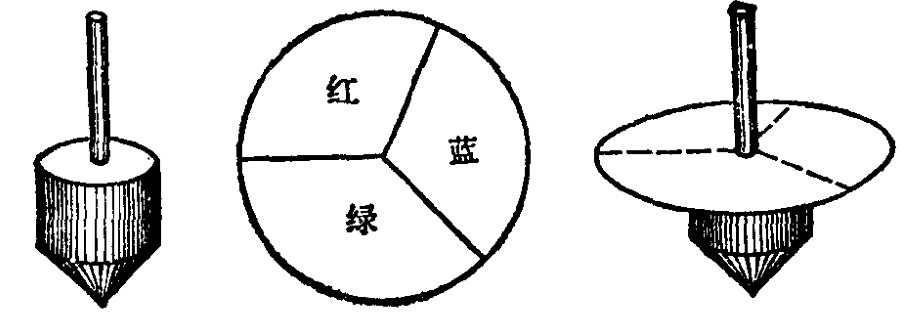
\includegraphics[width=0.6\textwidth]{../pic/czwl2-ch1-35}
    \caption{}\label{fig:1-35}
\end{figure}

如果改变三色板上三种颜色的深浅程度,当陀螺很快旋转的时候,看到三色板又是另一种颜色。
这样,调配红、绿、蓝三种颜色的深浅,我们便可以得到不同的颜色。



\section*{复习题}

(1) 什么现象可以说明光在同一种物质里传播的路线是直的?光在真空里的传播速度是多少

(2) 叙述光的反射定律。

(3) 平面镜里成的像跟物体是怎样的关系?

(4) 凹镜有什么重要的光学性质和应用?

(5) 当光从一种物质进入另一种物质的时候,折射光线跟入射光线有什么关系?

(6) 什么是凸透镜的主轴、焦点和焦距?

(7) 什么情况下凸透镜成实像?实像的位置和大小跟物体的所在位置有什么关系?

(8) 什么情况下凸透镜成虚像?虚像跟实像的区别是什么?

(9) 照相机、幻灯机、放大镜分别利用了凸透镜的哪种成像情况?

(10) 什么叫光的色散?

(11) 透明体的颜色是由什么决定的?不透明体呢?


